%===============================================================
% ICCAD 2014 submission
%
% ===============================================================

\documentclass[10pt,nocopyrightspace]{sigplanconf}

\usepackage{multirow}
\usepackage{amsthm}
\usepackage{amsmath}
\usepackage{amssymb}
\usepackage{empheq}
\usepackage{algorithm}
\usepackage[vlined,linesnumbered,ruled,algo2e]{algorithm2e}
\usepackage{color}
%\usepackage{subfigure}
\usepackage{subcaption}
\usepackage{booktabs}
\usepackage{url}
\usepackage[normalem]{ulem}
%\usepackage{subfig}
\usepackage{verbatim}
%\usepackage{listings}
\usepackage[caption=false,labelformat=simple]{subfig}
\usepackage{flushend}
\usepackage{paralist}
\usepackage{array}
\usepackage{enumitem}

\usepackage[compact]{titlesec}
\setlength\extrarowheight{1pt} % or whatever amount is appropriate

\newcommand{\fixme}[1]{\textcolor{red}{\small [~#1~]}}
\newcommand{\TT}[1]{\texttt{#1}}
\newcommand{\BF}[1]{\textbf{#1}}
\newcommand{\IT}[1]{\textit{#1}}
\newcommand{\RM}[1]{\textrm{#1}}
\newtheorem{lemma}{Lemma}
\newtheorem{theorem}{Theorem}

\newcommand{\interval}{T}
\newcommand{\latency}{L}

%%%%%%%%%%%%%%%%%%%%%%%%%%%%%%%%%%%%%%%%%%%%%%%%%%
\begin{document}
\renewcommand{\thesubfigure}{(\alph{subfigure})}
\title{ECE 5770 : Resilient Computer Systems \\
Surveying Efficient Low-Cost Memory Protection Techniques}

\authorinfo{Udit Gupta}
{School of Electrical and Computer Engineering, Cornell University, Ithaca, NY}
{ug28@cornell.edu}

\maketitle

\section{Introduction}
\label{sec-introduction}

%Define the problem and the goal of the project
%Explain why the problem is important
%Summarize your approach and key results
%Outline the rest of the paper

Since the advent of the Internet, computing devices have become not only more
prolific but also more varied - encompassing not only high performance
clusters but also general purpose computers and mobile systems.  Moreover, the
assumptions made about the security model of a system have changed drastically;
users can no longer be trusted, and devices have the potential to interact with
unknown and possibly untrustworthy hosts while communicating sensitive
information. For example, the boom in smartphones has caused a secondary
explosion in the mobile application industry, allowing users to log in to
various trusted systems (e.g. bank accounts, medical records and shopping
accounts) remotely.  The sudden increase in connectivity exposes users to
adversaries that may attempt to leverage these interactions in order to obtain
confidential information or disrupt the use of services or applications.

In response to these changes, there has been an increasing effort in developing
trusted computing platforms augmented with specialized hardware modules that
provide security features such as authentication and decryption/encryption. One
such security feature that remains a focus in trusted computing research is
protecting off-chip memory. One key component of protecting off-chip memory is
maintaining confidentiality of private data. Challenges in designing memory
protection mechanisms involves providing encryption primitives at a low cost
(money, area, power and design complexity), high throughput and low latency
without compromising security. Current work also focuses on memory protection
schemes for general purpose and high performance computing systems. The domain
of memory protection in the mobile and embedded computing domains is relatively
less studied and poses interesting challenges. Mobile and embedded devices
often operate under strict power and area constraints. Providing secure memory
protection while following the prescribed power and area constraints as well as
maintaining performance of the computing devices is an ongoing challenge.

According to Hollis \cite{hollis} there are two main source of power
consumption when driving I/O:

\paragraph{Dynamic A/C Power} Dynamic A/C power consumption from charging and
discharging capacitances (e.g. electrostatic discharge devices, driver output
capacitance, receiver input capacitance and the channel itself), is possibly
the dominant and most universal form of I/O power consumption. However, once
the capacitances have reached steady state, the dynamic a/c power consumption
is negligible. For the purposes of our study we assume that all device
capacitances are already in steady state - simplifying our model as we no
longer have to consider dynamic a/c power consumption.

\paragraph{Link Termination} The second most common source of I/O power
consumption is link termination schemes. Intuitively, when the driver
outputs a signal which is then received by the I/O device, a significant
portion of the signal is reflected back to the driver itself. Consequently, the
driver has to not only power the desired signal but also overcome the signal
reflections.  This incurs a significant power overhead. Past research in the
context of link termination schemes has focused on developing more efficient
DDR chip topologies to reduce signal reflections. For example, in Figure
\ref{dram-chips} illustrates the DDR2 and DDR3 DDR chip topologies. As driving
frequencies for DDR3 increased, memory architects adopted the fly-by network
topology which greatly reduces signal reflections and improves On-Die
Termination (ODT).

\begin{figure}[!htb]
  \centering
  \begin{subfigure}[b]{0.4\textwidth}
    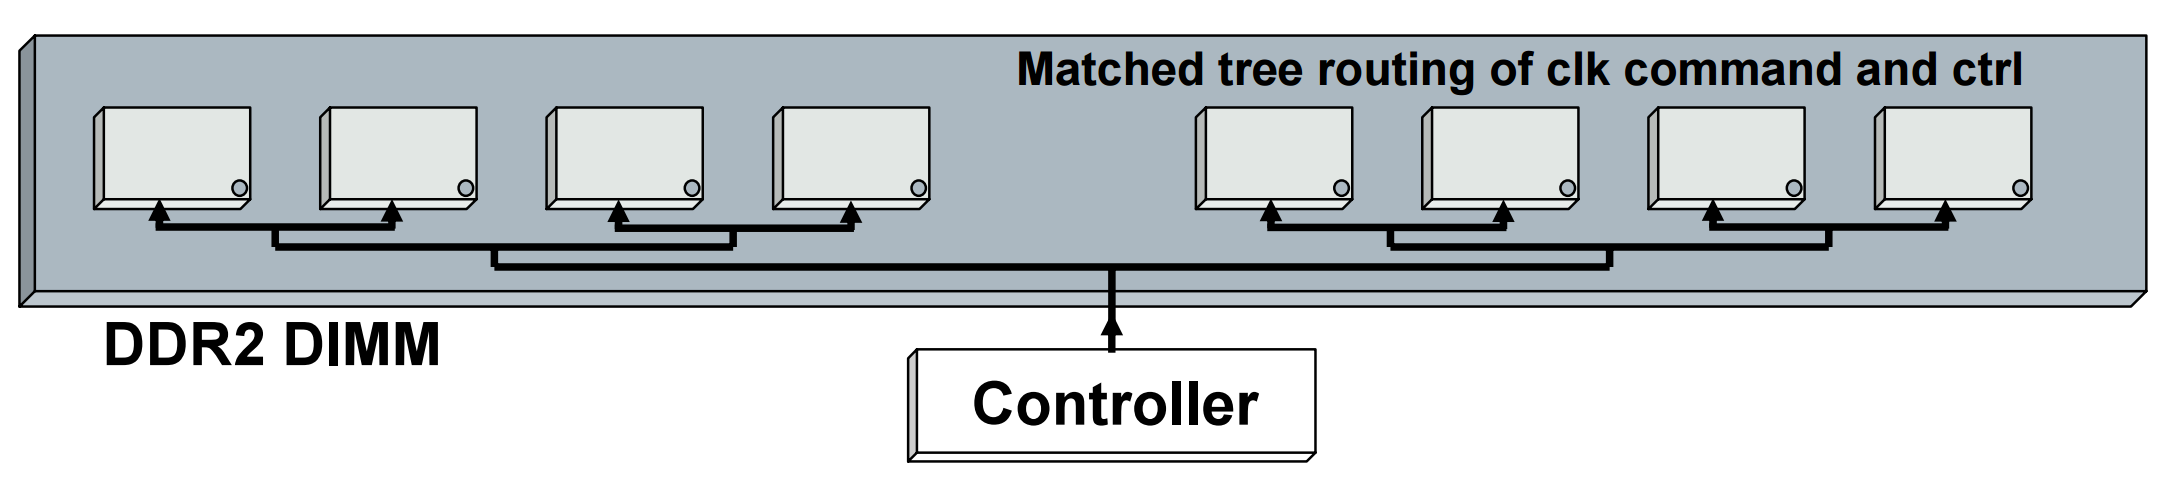
\includegraphics[width=\textwidth]{figs/ddr2-topology}
    \caption{Example DDR2 DRAM chip topology}
    \label{fig:ddr2-chips}
  \end{subfigure}

  \begin{subfigure}[b]{0.4\textwidth}
    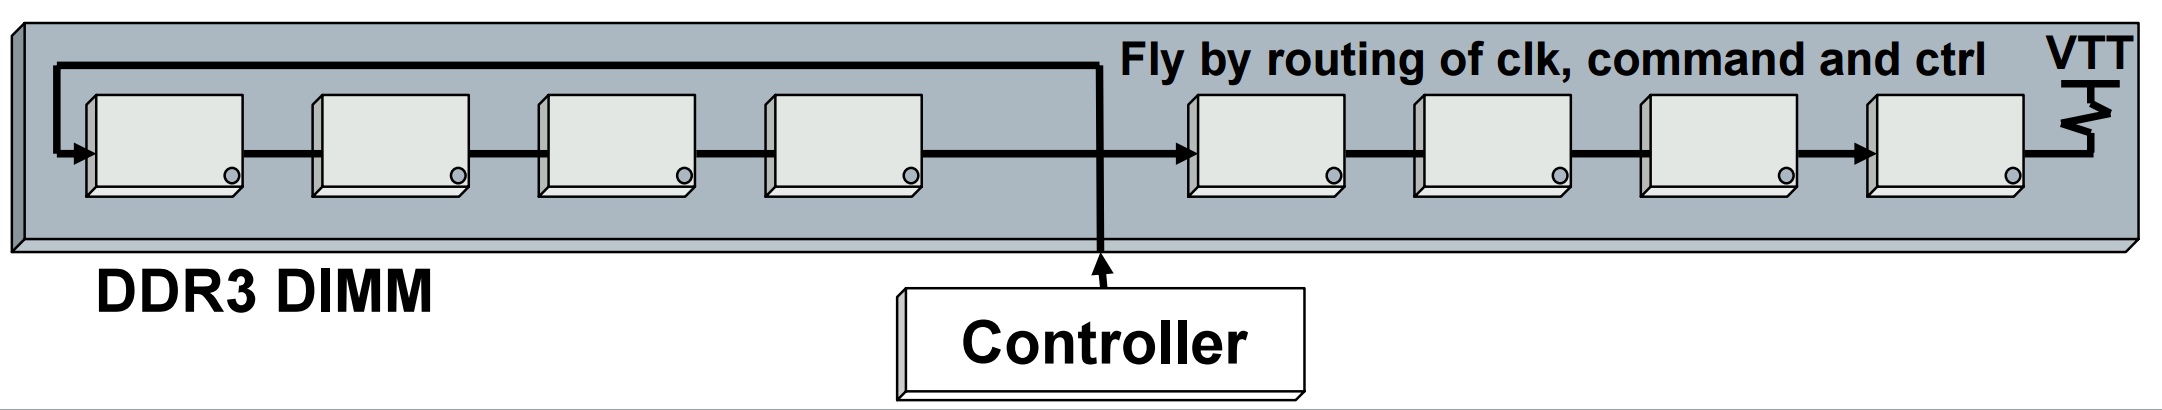
\includegraphics[width=\textwidth]{figs/ddr3-topology}
    \caption{Example DDR3 DRAM chip topology}
    \label{fig:ddr3-chips}
  \end{subfigure}
  \caption{Representative DRAM chip topologies for DDR2 and DDR3 memory
  technologies taken from \cite{ddr-design}}
  \label{dram-chips}
\end{figure}

Though existing DDR3 memory technologies implement more efficient DRAM chip
topologies to reduce signal reflections, ODT is still a prominent source of
power consumption. Memory architects are looking at more efficient read/write
schemes such as Data Bus Inversion (DBI) for further improving ODT power
consumption for DDR4. Our study focuses on using first order models for DBI
developed by Hollis \cite{hollis} in the context of memory encryption to
simulate the power overhead of secure memory encryption. Generally, our results
so that memory encryption does indeed incur a significant power overhead and
that DBI-DC and AC values for is relatively consistent across MiBench
applications.

The rest of this paper is organized as follows: Section~\ref{sec-problem}
outlines our general project goals and outlines the memory encryption model
used, Section~\ref{sec-methodology} outlines the high level model and
experimental setup for our study, Section~\ref{sec-evaluation} analyzes our
results and data, Section~\ref{sec-group-dynamics} reviews our group dynamic's
and work distribution, Section~\ref{sec-related} reviews related work in
relation to power consumption of secure memory encryption and
Section~\ref{sec-conclusions} concludes the paper with final remarks and future
work.

\section{Related Work}
\label{sec-related}

We organize the related work surrounding efficient, low-cost memory protection
techniques in two separate sections : \textbf{memory encryption} and
\textbf{memory integrity verification}.

\subsection{Memory Encryption}
The goal of memory encryption techniques is to protect the confidentiality of
sensitive information from unauthorized subjects. Sensitive information
includes : secret keys, secret code (e.g. proprietary boot code) and private
data. The \TT{National Institute of Standards and Technology} (NIST) actively
regulates the encryption standards. Recently, two symmetric key cryptographic
algorithms are being increasingly used in trusted computing : Triple Data
Encryption Standard (3DES) and Advanced Encryption Standard/Rjindael (AES). As
AES provides systems with a higher minimum security strength, it is more widely
used in recent hardware accelerated trusted computing studies as compared to
3DES. For instance, Intel has developed extensions to it's instruction set
architecture (ISA) to enable fast encryption and decryption using AES. The
studies in this survey focus on using AES to develop efficient, low-cost
encryption and decryption modules.

%%%%%%%%%%%%%%%%%%%%%%%%%%%%%%%%%%%%%%%%%%%
\subsubsection{AES Counter Mode Encryption}
%%%%%%%%%%%%%%%%%%%%%%%%%%%%%%%%%%%%%%%%%%%
AES supports three general modes of operation: Electronic Codebook (ECB),
Cipher Block Chaining (CBC) and Counter (CTR). Since the AES-ECB mode preserves
patterns from the plaintext to the ciphertext, it does not provide adequate
confidentiality protection. Both AES-CBC and AES-CTR eliminate this information
leak by chaining the encryption between blocks. This however precludes users
from encrypting and decrypting blocks in parallel (as supported by AES-ECB). As
discussed in \cite{suh-memIntEnc}, decrypting the ciphertext stored in memory
can drastically increase the load use delay latency of processing systems. The
added latency is a result of the serial : fetch memory then decrypt memory
block operation. To hide this latency Suh et. al. use a \TT{one-time pad} (OTP)
based encryption / decryption technique. The OTP is generated by encrypting the
plaintext = {\TT{FV} $||$ \TT{Addr} $||$ \TT{TS} $||$ \TT{i}}, under a secret
key using AES-CTR. \TT{FV} is a fixed vector, \TT{Addr} is the memory address
being accessed, \TT{TS} is a timestamp stored along with the encrypted data and
\TT{i} is the block number. The use of a monotonically incrementing counter,
\TT{TS}, ensures the uniqueness of the \TT{OTP} which is then proven to be
secure. Generating the \TT{OTP} using this method enables the system to overlap
the AES-CTR decryption latency with the memory fetch / accessing latency
\cite{suh-memIntEnc}. Suh et. al. also mentions the \TT{TS} values can be
cached to mitigate the memory access latency for fetching the \TT{TS} and
better hiding the AES-CTR decryption latency. This method reduces the
load-use-delay latency to the latency of performing an $\oplus$ between the
generated \TT{OTP} and encrypted data.

%%%%%%%%%%%%%%%%%%%%%%%%%%%%%%%%%%%%%%%%%%%
\subsubsection{AEGIS}
%%%%%%%%%%%%%%%%%%%%%%%%%%%%%%%%%%%%%%%%%%%
Furthering the AES-CTR based decryption \cite{suh-memIntEnc}, AEGIS
\cite{aegis} adds low-level OS-kernel support to provide additional
confidentiality features. AEGIS, a single-chip secure processor, leverages
OS-kernel modes to provide additional encryption (ME mode) and
integrity-verification (IV mode) features. The OS also manages four distinct
protected regions in virtual memory

\begin{enumerate}[noitemsep, topsep=0pt]
    \item Read-only (static) verified memory
    \item Read-write (static) verified memory
    \item Read-only (dynamic) private memory
    \item Read-write (dynamic) private memory
\end{enumerate}

These modes help isolate the virtual memory space of each process to ensure
that secret keys are kept confidential across multiple users and between users
and the supervisor. AEGIS also employs physically random functions (also called
physically unclonable functions) to secret keys as they are less prone to
physical hardware attacks than the alternatives such as using non-volatile
memory (e.g. EEPROM) and fuses.

%%%%%%%%%%%%%%%%%%%%%%%%%%%%%%%%%%%%%%%%%%%
\subsubsection{Duece}
%%%%%%%%%%%%%%%%%%%%%%%%%%%%%%%%%%%%%%%%%%%

Thread Model : Snooping and DIMM read attack

Need to consider the following:
\begin{enumerate}
  \item Without encryption, most writes only change around 12 \% of bits.
  \item \textbf{Avalance Effect} \cite{avalance} - Even changing 1 bit can
    change the entry encrypted bitstring : 1 bit causes 50\% of bits on average
    to change.
  \item Cannot use techniques such as \TT{Data Comparison Write} \cite{dcr} and
    \TT{Flip-n-Write} \cite{fnw} to reduce bit's written.
  \item This affects power consumption as now all the bits must be written.
  \item This affects write durability of memory as memory writes will causes
    memory to wear out faster (more bits written - 4x more on average)
\end{enumerate}
Used non-volatile memory (PCM).
\begin{enumerate}
  \item Dual Counter Encryption : Leading and Trailing Counters.
  \item Only encrypt modified elements under Leading counter and everything
    else using trailing counter.
  \item This reduces memory writes from 50 \% to 24 \% on average.
  \item Also enable the option to dynamically swtich to \TT{Flip-n-Write} mode
    if all the bits in the chance block / line are changing.
  \item Decrease power significantly.
  \item Only have the added overhead of 1 bit per encryption level. Tells if
    the block was encrypted in the current Epoch.
  \item To eliminate wear leveling (only certain cache blocks being written to
    usually) they also implemented an efficient horizontal wear leveling
    technique that uses algebraic functions to calcuate the rotation level.
\end{enumerate}

\subsubsection{GCM Based}
The GCM based approach \cite{gcmMem} uses a split counter mode in this
encryption and decryption routines. The split counter maintains two counters :
major and minor counter. The major counter is unqiue per encryption page and
minor counter per block. There are appoximately 8 bits in the minor counter and
64 bits in the major counter. The major and minor are concatenated to make the
counter for the encryption. GCM is secure like AES and highly efficient /
parallel.

%%%%%%%%%%%%%%%%%%%%%%%%%%%%%%%%%%%%%%%%%%%%%%%%%%%%%%%%%%%%%%%%%%%%%%%%%%%%%%%
\subsection{Integrity}
%%%%%%%%%%%%%%%%%%%%%%%%%%%%%%%%%%%%%%%%%%%%%%%%%%%%%%%%%%%%%%%%%%%%%%%%%%%%%%%
\subsection{Merkle}
Merkle trees \cite{merkle} are the idea of using a hash tree to store the
authentication tags and reduce the \TT{integrity check} from a linear
relationship of the number of memory operation to a logarithmic one. Many
techniques have been used to reduce the architectural overhead of this
including the arity of the hash tree, the granularity of the authentication and
maintaining a cache for the hashes. This can be problematic though as
maintaining the cache is complex and if it is combined with the data cache, it
can severely increase miss rates and pollute the cache. Also, an efficient
improvement is to only check until a node is the cache tree that is known to be
trusted is verified (which is in the cache).

\subsubsection{Suh - Efficient Memory Integrity and Encryption}
Mainly focuses on integrity with log based hash tables. It keeps a log of a
sequence of memory operations to maintain a snapshot of the current state of
the memory. This is considered \TT{lazy} memory integrity management because it
only detects the malliciously modified memory much after the attack (possibly)
since the authentication scheme only acts very intermittently.

\TT{Integrity verification} - Cache Hash Tree approach or the Log based
  approach discussed in \cite{suh-memIntEnc}. Log based is more efficient in
  terms of performance and space requried.

\subsubsection{Suh - AEGIS}
Develops a single-core processor extension, AEGIS, \cite{aegis} to provide
security features. AEGIS leverages Physical Random Functions (PRF) and off-chip
memory protection. For memory integrity protection there is defined by specific
operating modes (PTR and TE). Memory pages can be defined to be under
plaintext, integrity, confidentiality and or both protection.

\subsubsection{GCM Based}
The GCM based approach uses the GMAC / GHASH functions to provide memory
authentication capabilities. They do not use MD-5 or SHA-1, SHA-2 as they are
much more computationally intensive and incur a high latency. They use the idea
of Merkle trees to do the \TT{integrity} check but hide the fetch latency using
caches and authentication computation. The authentication also generates pads
which can be hidden in the memory access latency and finally XOR's these pads
with the data (plaintext for authenticated and ciphertext for verifying) like
the counter mode. Parallelize the Merkle tree to hide that latency as well.

\subsubsection{Multi-Core}
The multicore paper \cite{multicoreEnc} discusses how traditional Merkle tree
approaches do not work for multiprocessor systems. They instead have a single
global MAC tree managed by the memory controller. They also rely on having a
secure OS kernel which manages session keys which are used to generate secret
keys.

\section{Strengths and Weaknesses of Existing Work}
\label{sec-discussions}

\subsection{Suh - Efficient Memory Integrity and Encryption}
This paper explores efficient memory integrity verification techniques and
encryption techniques separately. It does not consider the increased power and
overhead associated with memory writes after encryption as discussed in the
following section by Duece.

\subsection{Duece}
\cite{duece} focuses on PCM (non-volatile) memory encryption and devises a
low-cost technique that is applicable to most systems - reducing the overhead
of memory writes. It uses a wide array of benchmarks (namely SPEC). It also
proposes a novel wear-leveling approach that prolongs memory lifespan. It
protects only confidentiality but not integrity. It requires 2 AES engines (1
for modified words and another for unmodified words).

\section{Conclusion}
\label{sec-conclusions}

Generally our study hopes to make a small step in developing a reliable model
for power consumption overheads of secure memory systems. Where previous
studies have either focused on performance and area or non-volatile memory
systems, our system investigates power consumption of traditional DDR based
memory technologies --- namely DDR4. Focusing on DBI-enabled memory systems, we
have developed a simulation infrastructure that can be used to model the
affects of encrypted data on ODT power consumption resulting from link
termination and signal reflections. In theory, this model could be used for a
wide array of I/O devices that support DBI, or similar schemes. We leverage
Pin, a dynamic instrumentation tool for computer architecture simulations and
MiBench as a representative set of mobile workloads. We find that encryption,
as expected, does incur a significant power overhead on DBI-enabled off-chip
memory systems.

In the future we hope to develop a real computing system with a DBI-enabled
off-chip memory system and verify our models and collect empirical data from
the prototype. This would would also enable researchers to measure system-wide
power metrics for improving secure processor designs. We also hope to
investigate alternative write schemes to DBI --- especially ones targeting
encrypted read and write operations. Finally, we hope that one day a single
unified model or infrastructure for simulating the performance, area and power
consumption of real mobile computing systems is developed to facilitate more
productive design space explorations of secure mobile computing.


% references section
%\newpage

\bibliographystyle{abbrv}
\bibliography{bib/hls,bib/compile,bib/security}

\end{document}


